% This version of CVPR template is provided by Ming-Ming Cheng.
% Please leave an issue if you found a bug:
% https://github.com/MCG-NKU/CVPR_Template.

% \documentclass[review]{cvpr}
\documentclass[final]{cvpr}

\usepackage{times}
\usepackage{epsfig}
\usepackage{graphicx}
\usepackage{amsmath}
\usepackage{amssymb}

% Include other packages here, before hyperref.

% If you comment hyperref and then uncomment it, you should delete
% egpaper.aux before re-running latex.  (Or just hit 'q' on the first latex
% run, let it finish, and you should be clear).
\usepackage[pagebackref=true,breaklinks=true,colorlinks,bookmarks=false]{hyperref}


\def\confYear{CVPR 2021}
%\setcounter{page}{4321} % For final version only


\begin{document}

%%%%%%%%% TITLE
\title{The Report of the Assignment 2:\\Implementing and Reproducing MAML and REPTILE}

\author{Seungmin Lee\\
Seoul National University\\
{\tt\small dltmdals14@snu.ac.kr}
}

\onecolumn
\maketitle


%%%%%%%%% BODY TEXT
\section{Introduction}
In this assignment, I implemented and reproduced MAML~\cite{maml}, FOMAML~\cite{maml}, and Reptile~\cite{reptile}. I followed the instructions for all experiments. Therefore, I skip all the details of the experiments. In the following section, I report the results of each task using the required graphs.

\section{Omniglot Classification Results}~\label{omniglot}
In Omniglot~\cite{omniglot} experiments, we compare just FOMAML~\cite{maml} and Reptile~\cite{reptile}. Figure~\ref{comp2} display the results of the experiments. As we can see in the figure, 1-shot and 5-shot results are similar in that they converge very fastly. However, the starting losses are quite different. More specifically, in 1-shot classification tasks, the starting loss of FOMAML is between 4 and 5, while that of 5-shot classification is larger than 7. On the other hand, the results of Reptile show similarities in both experiments. The final losses of FOMAML are smaller than that of Reptile. Moreover, the accuracies of FOMAML are larger than Reptile. The final accuracies of FOMAML are 92.29 and 96.58 for 1-shot and 5-shot classification, respectively, while the final accuracies of Reptile are only 87.21 and 87.30.

In all experiments, we used ten tasks, 5 inner steps, 50 test inner steps, and 20000 epochs, while we changed meta LR and inner LR. More specifically, we used 0.001 and 0.4 as meta LR and inner LR, respectively, for training 1-shot and 5-shot FOMAML. For 1-shot and 5-shot Reptile, we used 0.001 and 0.1 as meta LR and inner LR, respectively.

\begin{figure}[b]
    \centering
	\begin{tabular}{c}
		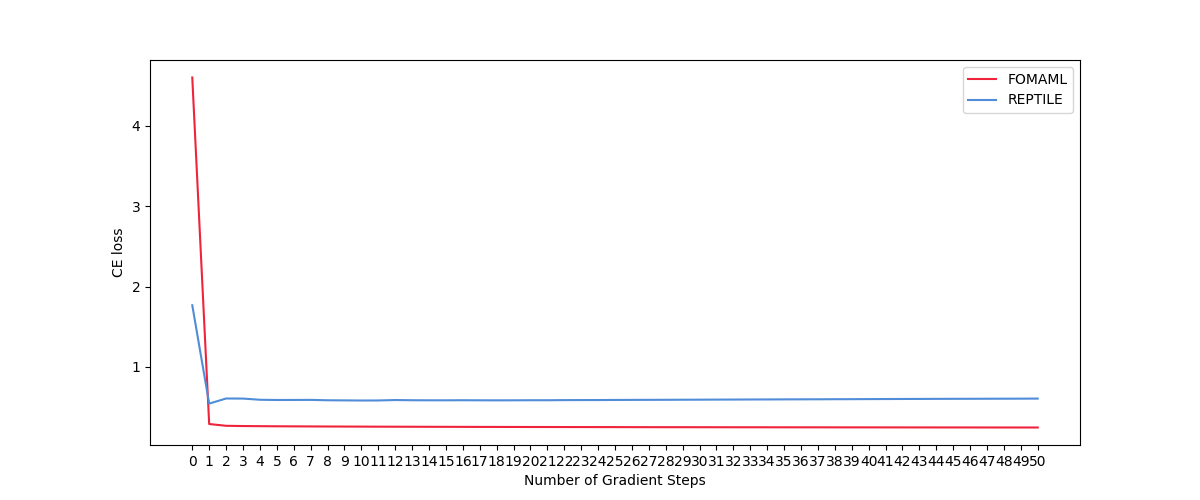
\includegraphics[width=0.9\textwidth]{resources/omniglot_5way_1shot.png}\\
		(a) 5-way 1-shot classification\\
		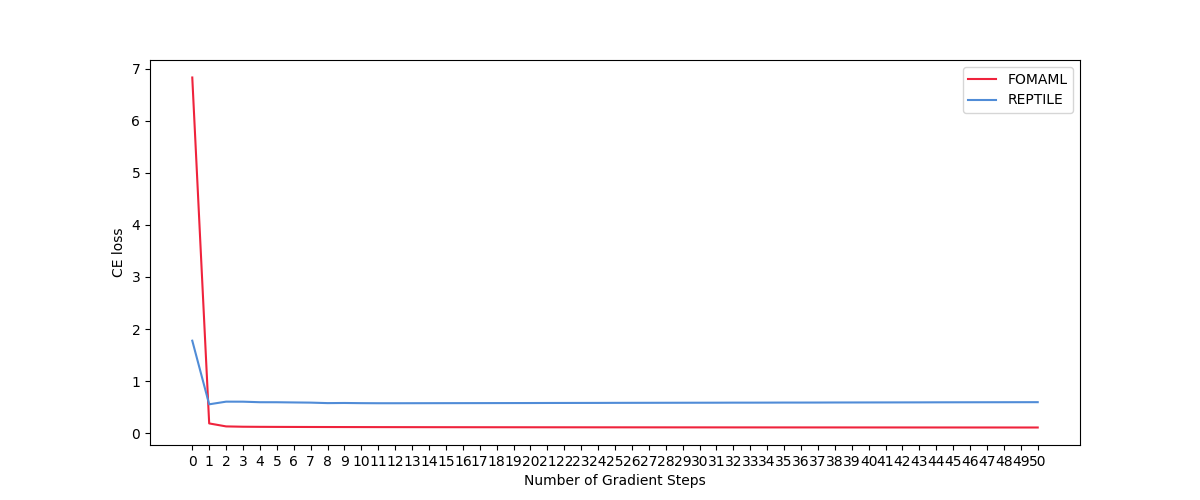
\includegraphics[width=0.9\textwidth]{resources/omniglot_5way_5shot.png}\\
		(b) 5-way 5-shot classification\\
	\end{tabular}\vspace{0.2cm}
	\caption{The results of (a) 5-way 1-shot classification and (b) 5-way 5-shot Omniglot classification.}
	% \vspace{-0.4cm}
	\label{comp2}
\end{figure}


\section{Sine Waves Regression Results}
For this regression experiments, we tested MAML~\cite{maml}, FOMAML~\cite{maml}, and Reptile~\cite{reptile}. In all experiments, we used 10000 epochs, 10 test inner steps, and we used the same meta LR and inner LR for the same algorithms. For training MAML and FOMAML, We used \{0.001, 0.0001, 1, 1000\} as \{meta LR, inner LR, inner steps, tasks\}, respectively. We used \{0.001, 0.01, 5, 100\} as \{meta LR, inner LR, inner steps, tasks\} for training Reptile.

The results are shown in Figure~\ref{sin5} and Figure~\ref{sin10}. For 5-shot tasks, the training loss of FOMAML seems unstable but eventually converges. The other losses decrease monotonically in all experiments. MAML shows the best results for all experiments, while it uses the most resources when calculating second-order gradients.

\begin{figure}[b]
    \centering
	\begin{tabular}{c}
		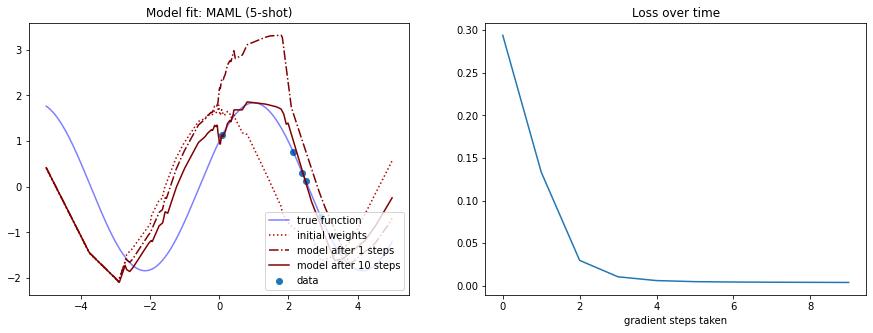
\includegraphics[width=0.9\textwidth]{resources/maml_5.png}\\
		(a) MAML (5-shot) \\
		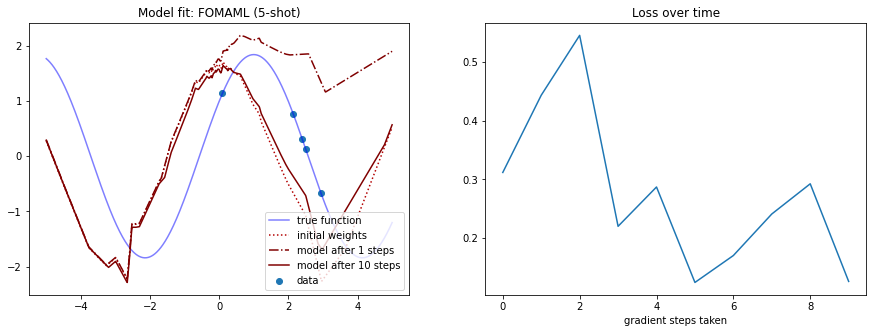
\includegraphics[width=0.9\textwidth]{resources/fomaml_5.png}\\
		(a) FOMAML (5-shot) \\
		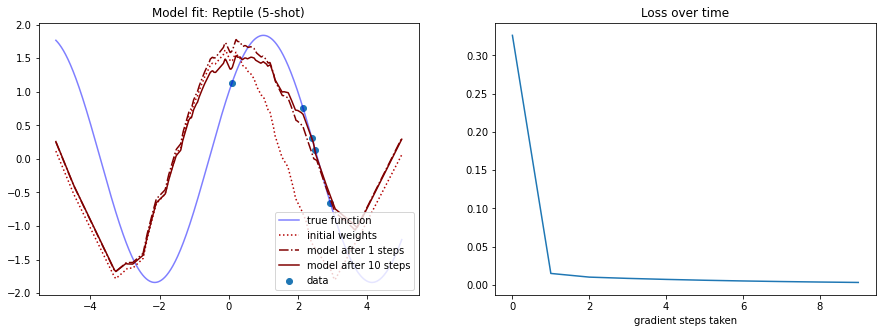
\includegraphics[width=0.9\textwidth]{resources/reptile_5.png}\\
		(a) Reptile (5-shot) \\
	\end{tabular}\vspace{0.2cm}
	\caption{The results of 5-shot sine waves regression tasks.}
	% \vspace{-0.4cm}
	\label{sin5}
\end{figure}

\begin{figure}[b]
    \centering
	\begin{tabular}{c}
		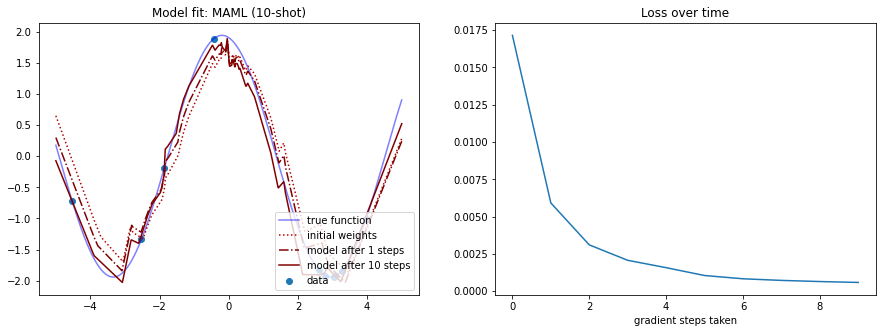
\includegraphics[width=0.9\textwidth]{resources/maml_10.png}\\
		(a) MAML (10-shot) \\
		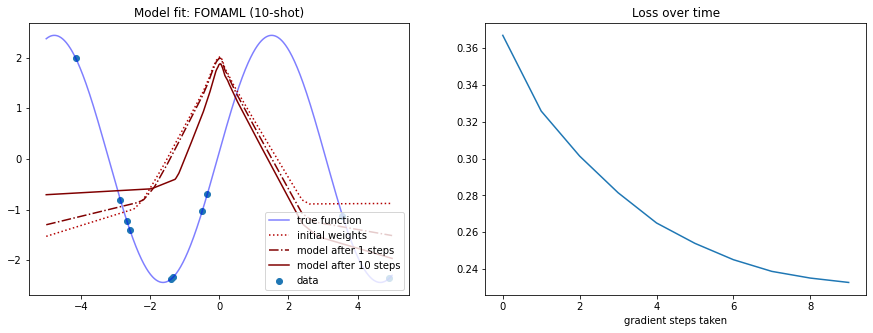
\includegraphics[width=0.9\textwidth]{resources/fomaml_10.png}\\
		(a) FOMAML (10-shot) \\
		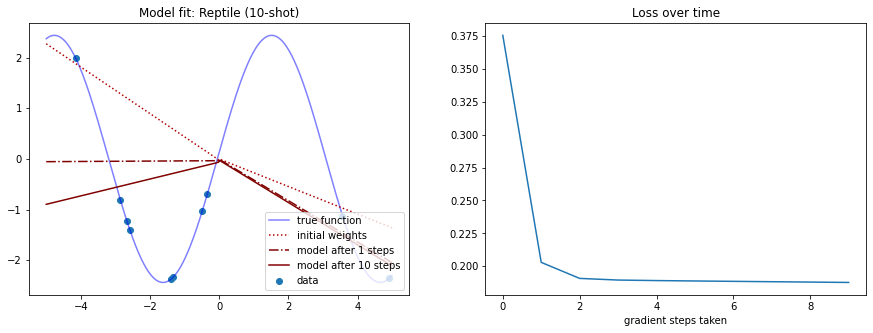
\includegraphics[width=0.9\textwidth]{resources/reptile_10.png}\\
		(a) Reptile (10-shot) \\
	\end{tabular}\vspace{0.2cm}
	\caption{The results of 10-shot sine waves regression tasks.}
	% \vspace{-0.4cm}
	\label{sin10}
\end{figure}

{\small
\bibliographystyle{ieee_fullname}
\bibliography{egbib}
}

\end{document}
